
\chapter{Przegląd systemów rekomendacyjnych}

Systemy rekomendacyjne pomagają użytkownikom w zdobyciu wartościowych i spersonalizowanych informacji z dużego źródła danych. Większość przypadków działania takiego systemu opiera się na przewidzeniu preferencji użytkownika na podstawie wcześniej zgromadzonych danych.

Ważnym momentem w historii systemów rekomendacyjnych był otwarty konkurs \textit{Netflix Prize} polegający na zaproponowaniu najlepszego algorytmu \textit{collaborative filtering} mającego na celu przewidzenie oceny filmu danej przez użytkownika, opierając się wyłącznie na poprzednich ocenach, bez dodatkowych informacjach o użytkownikach i filmach. W tym celu opublikowano zbiór testowy zawierający ponad 100 milionów ocen wystawionych przez 500 tysięcy anonimowych użytkowników. W wyzwaniu wzięło udział ponad 48 tysięcy zespołów z 182 państw [2].

Po konkursie \textit{Netflix Prize} głównym motywem przewodnim w pracach naukowych stała się faktoryzacja macierzy. Również w celu zwiększenia skuteczności algorytmu uwagę poświęcono takim zagadnieniom jak: wykorzystanie sieci społecznościowych oraz uczenia głębokiego w systemach rekomendacyjnych [1].

Rozdział omawia sposób działania systemów rekomendacyjnych, główne problemy i wyzwania stawiane tym systemom. Także przedstawiono popularne mechanizmy, sposoby ewaluacji oraz główne zalety poszczególnych rozwiązań.

\section{Założenia systemów rekomendacyjnych}

Głównymi zadaniami systemów rekomendacyjnych jest odfiltrowanie przedmiotów (na przykład: filmy, książki), które są dla użytkownika potencjalnie mało interesujące lub nieatrakcyjne. Użytkownik korzystający z serwisu wspieranego przez tego typu systemy otrzymuje jako proponowane, mały, spersonalizowany zestaw produktów z całego zbioru.

Systemy rekomendacyjne mogą zostać podzielone na dwie grupy ze względu na podejście [1]: spersonalizowane oraz niespersonalizowane. Pierwsze opierają swoje działanie na zebranych danych użytkownika. Informacje o odwiedzających mogą zostać zdobyte poprzez monitorowanie zachowań użytkowników lub poprzez bezpośrednie zapytanie użytkowników o ich preferencje. Natomiast podejście niespersonalizowane bazuje na zachowaniach pozostałych użytkowników.

Dane zazwyczaj przedstawiane są w formie dwuwymiarowej macierzy $R = U \times I$, gdzie U jest to zbiór n użytkowników oraz I zbiór m przedmiotów. Tabela \ref{macierzUI} przedstawia przykład takiej macierzy, wiersze reprezentują użytkowników, kolumny przedmioty, oceny są w przedziale 1 do 5, natomiast 0 oznacza brak oceny. Aby uzyskać lepsze rekomendacje systemy mogą wykorzystać macierze o większej liczbie wymiarów (zawierających czas, lokalizację czy informacje uzyskane z mediów społecznościowych).

Dzięki coraz lepszym technikom zdobywania danych oraz spadającej tendencji do udzielania ocen wśród klientów, popularnym stało się wykorzystanie domniemanych danych (\textit{ang. implict data}) takich jak: liczba kliknięć lub wyświetleń do budowania akademickich oraz branżowych systemów rekomendacyjnych \cite{Adomavicius2005}. Dane takie w przeciwieństwie do informacji sprecyzowanych (\textit{ang. explict data}) nie opierają się o negatywne sprzężenie zwrotne oraz nie wymagają metryki pewności (nawiązują do częstotliwości występowania zjawiska).

\label{macierzUI}
\begin{table}[h]
\centering
\caption{Przykład macierzy użytkownik-przedmiot.}
\begin{tabular}{|c|c|c|c|c|c|}
\hline
&
Przedmiot1 &
Przedmiot2 &
Przedmiot3 &
Przedmiot4 &
Przedmiot5
\\
\hline
  
Użytkownik1 &
1 &
5 &
4 &
2 &
3
\\
\hline
  
Użytkownik2 &
5 &
0 &
2 &
4 &
0
\\
\hline

Użytkownik3 &
1 &
0 &
4 &
0 &
4
\\
\hline

Użytkownik4 &
3 &
0 &
3 &
1 &
5
\\
  \hline

Użytkownik5 &
2 &
0 &
2 &
0 &
3
\\
\hline
\end{tabular} 
\end{table}

Ze względu na rodzaj wyjścia (otrzymanego wyniku) systemy rekomendacyjne możemy podzielić na następujące dwie grupy: pojedyncza predykcja oraz top-N predykcji. Pierwsza polega na przewidzeniu dokładnej oceny, którą użytkownik mógłby dać przedmiotowi, natomiast drugie podejście zwraca N nieocenionych przedmiotów, które mogłyby najbardziej przypaść do gustu użytkownikowi.


\section{Problemy i wyzwania}

Rzadkość danych - następuje w momencie, gdy wielu użytkowników oceniło tylko kilka przedmiotów przez co system rekomendacyjny nie może poznać preferencji użytkownika (macierz użytkownik-przedmiot ma zbyt wiele pustych wartości).

Skalowalność - systemy rekomendacyjne wraz ze wzrostem liczby użytkowników muszą radzić sobie z napływem coraz większej liczby danych do przetworzenia. Gdy takie dane wynoszą miliony użycie standardowych mechanizmów rekomendacyjnych może powodować otrzymanie wyników rekomendacji z dużym opóźnieniem (niewystarczający krótki czas na uzyskanie odpowiedzi). Bardziej złożony system wymaga większej liczby osób usprawniających oraz zarządzających jego działaniem, co równa się większemu kosztowi utrzymania zarówno pracowników jak i sprzętu komputerowego na którym taki system jest wdrożony.
    
Czarna owca - zjawisko występuje w momencie, gdy preferencje jednego z użytkowników nie pokrywają się z wyodrębnionymi grupami użytkowników, stąd użytkowników nie będzie w stanie otrzymać spersonalizowanych rekomendacji.

Długi ogon - następuje w momencie, gdy rekomendacja opiera się na produktach podobnych do siebie. Wtedy użytkownicy oglądają tylko część oferowanych przez serwis przedmiotów. Zjawisko to objawia się tym, że produkty, które potencjalnie mogą się podobać konsumentowi nie zostaną mu zaprezentowane.

Zimny start (ang \textit{cold-start)} - występuje w momencie rejestracji do systemu nowego użytkownika lub przedmiotu. Przedmioty nie mogą zostać zarekomendowane, ponieważ nie mają żadnej oceny natomiast nowi klienci dokonali zbyt mało ocen.

\section{Content-based filtering}
\textit{Content-based filtering} oparte jest na założeniu, że użytkownik polubi przedmioty o podobnej charakterystyce do tych, które poprzednio zostały przez niego polubione (schemat działania przedstawiony na rys. \ref{fig:content-based}). Do tego celu wykorzystywane są opisy produktów (na przykład przedstawione w formie tagów) do generowania rekomendacji. Plusem tego podejścia jest fakt, że do przeprowadzenia rekomendacji nie są potrzebne dane użytkownika, jednak wymagany jest dokładny opis oraz cechy charakterystyczne danego produktu. Przykładami takich cech może być zawartość książki lub sygnał akustyczny utworu muzycznego.

\begin{figure}
    \centering
    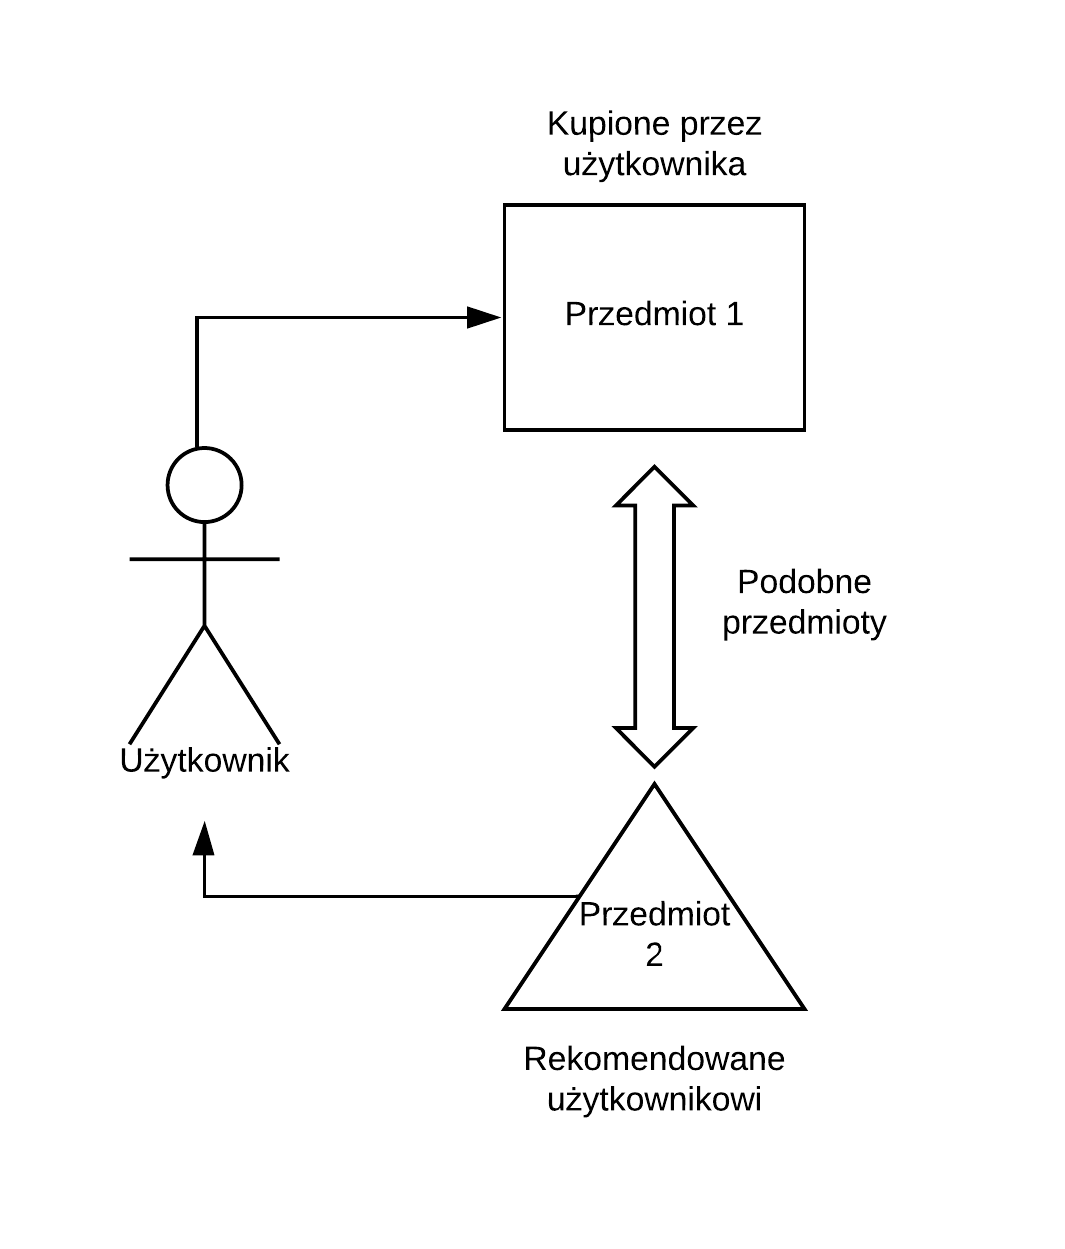
\includegraphics{images/content-based.png}
    \caption{Sposób działania mechanizmu \textit{Content-based filtering}.}
    Źródło: opracowanie własne na podstawie \cite{challenges_solutions_survey}
    \label{fig:content-based}
\end{figure}

\section{Collaborative filtering}

Podejście to nie wykorzystuje cech charakterystycznych przedmiotu (tak jak to było w metodzie \textit{Content-based filtering}), jednak problemem jest wygenerowanie rekomendacji dla nowego użytkownika lub produktu (\textit{cold start}). Metoda ta stosowana jest w dużych, komercyjnych aplikacjach. Ma wiele dobrze poznanych, różnorodnych algorytmów i wariacji przez co stosowana jest w wielu domenach.

Opisywana metoda może zostać podzielona na dwie podkategorie:

\begin{itemize}
    \item podejście pamięciowe (\textit{ang. memory based}) rekomenduje przedmiot na podstawie zbioru poprzednio ocenionych przez użytkownika przedmiotów. Dla przykładowego użytkownika \textit{u}, predykcja wyliczana jest na podstawie podobnych do niego użytkowników (główna idea przedstawiona na rys. \ref{fig:collaborative}) lub przedmiotów podobnych do tych, które wcześniej ocenił. Miara podobieństwa najczęściej obliczana jest korelacją Pearsona lub podobieństwem kosinusowym,
    \item podejście modelowe (\textit{ang. content based}) wykorzystuje dane historyczne. Jedną z najczęściej stosowanych metod w tym podejściu jest faktoryzacja macierzy, która zakłada, że użytkownicy oceniają przedmioty na podstawie pewnych cech. W przypadku muzyki może być jej gatunek lub wykonawca. W takim przypadku system rekomendacyjny jest w stanie odkryć czynniki umożliwiające na lepszą skuteczność systemu (liczba czynników powinna być mniejsza od liczby użytkowników i przedmiotów). 
\end{itemize}

W celu określenia miary podobieństwa pomiędzy użytkownikami najczęściej stosowana jest korelacja Pearsona. Definiowana jest ona w następujący sposób:

\begin{equation}
Pearson(x,y) = \frac{\sum\limits_{i=1}^n(x_i - \overline{x})(y_i - \overline{y})}{\sqrt{\sum\limits_{i=1}^n(x_i - \overline{x})^2}\sqrt{\sum\limits_{i=1}^n(y_i - \overline{y})^2}},
\end{equation}
dla podobieństwa dwóch użytkowników wzór wygląda następująco:

\begin{equation}
Pearson(a,b) = \frac{\sum\limits_{p \in P}(r_{a,p} - \overline{r}_a)(r_{b,p} - \overline{r}_b)}{\sqrt{\sum\limits_{p \in P}(r_{a,p} - \overline{r}_a)^2}\sqrt{\sum\limits_{p \in P}(r_{b,p} - \overline{r}_b)^2}},
\end{equation} gdzie:
\begin{itemize}
    \item a,b -- użytkownicy,
    \item $r_{a,p}$ -- ocena użytkownika a dla przedmiotu p,
    \item $r_{b,p}$ -- ocena użytkownika b dla przedmiotu p,
    \item $\overline{r}_a$ -- średnia ocen użytkownika a,
    \item $\overline{r}_b$ -- średnia ocen użytkownika b,
    \item P -- zbiór przedmiotów ocenionych przez obu użytkowników.
\end{itemize}

Uzyskane w ten sposób wartości są z przedziału [-1; 1], im wyższa liczba tym użytkownicy są do siebie bardziej podobni.

\begin{figure}
    \centering
    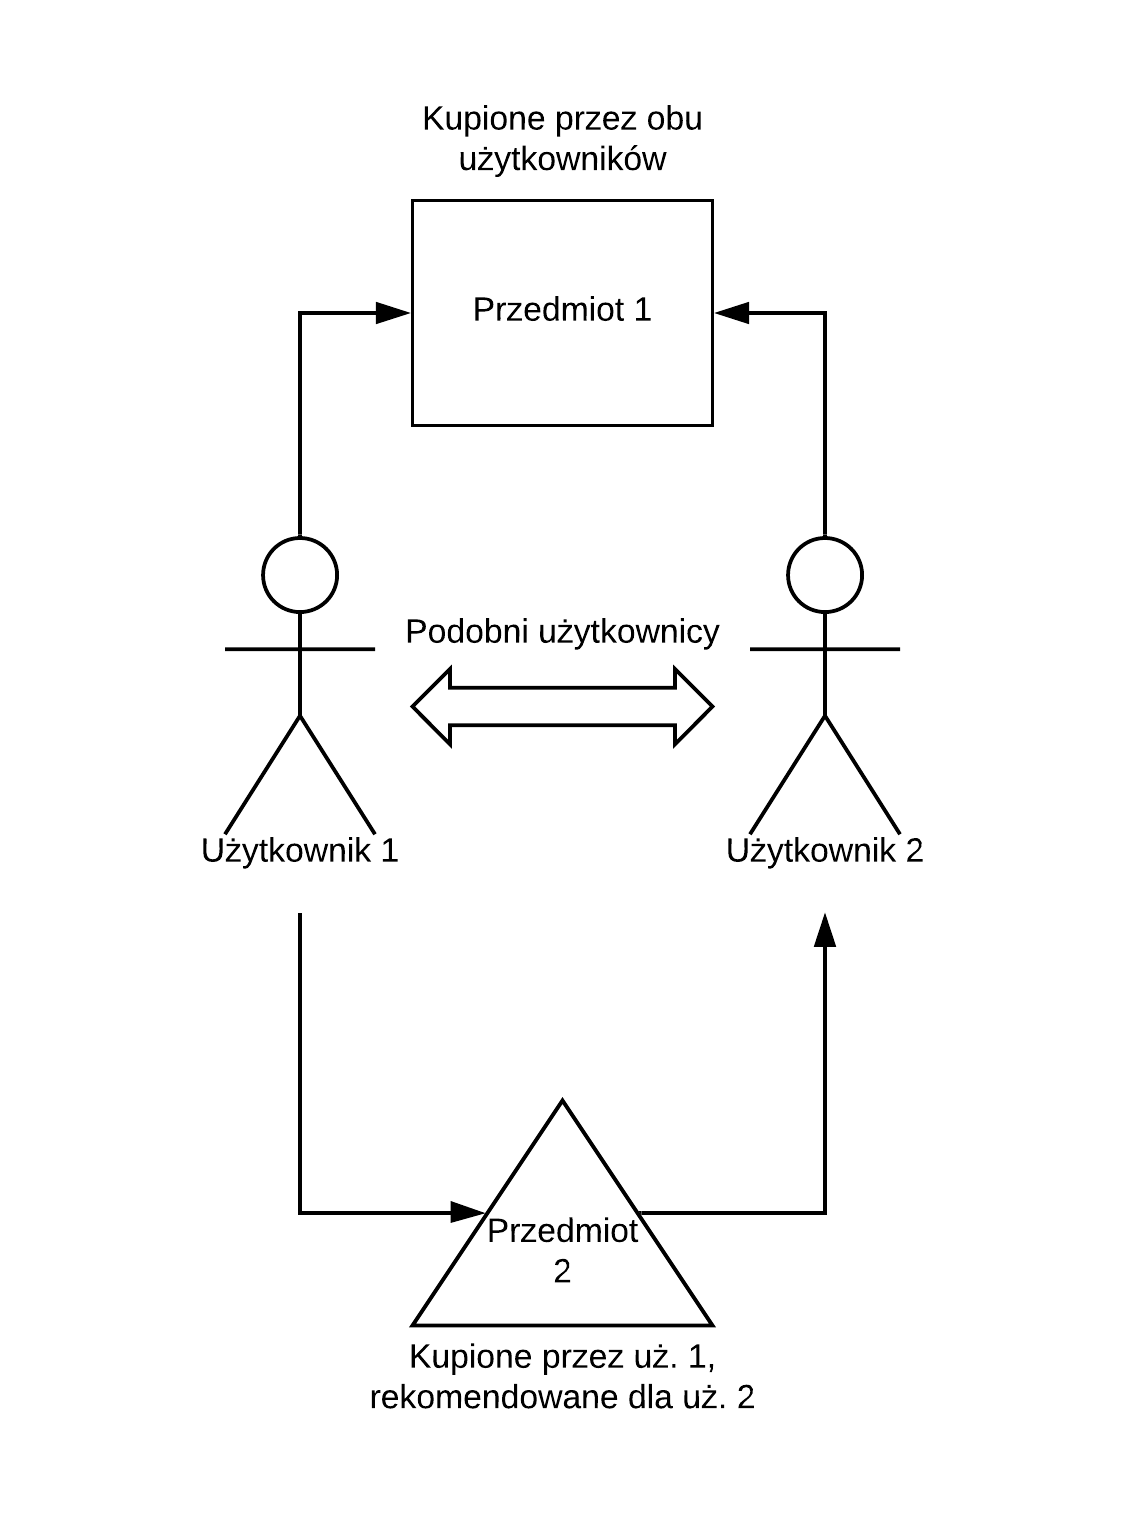
\includegraphics[scale=0.7]{images/collaborative.png}
    \caption{Sposób działania mechanizmu \textit{Collaborative filtering}.}
    Źródło: opracowanie własne na podstawie \cite{challenges_solutions_survey}
    \label{fig:collaborative}
\end{figure}

\section{Knowledge-based filtering}

Podejście oparte o wiedzę swoje działanie na wykorzystaniu źródeł wiedzy, które nie zostały uzyskane za pomocą poprzednio omawianych metod. Rekomendacje generowane są na podstawie wiedzy dziedzinowej preferencji użytkownika, cech przedmiotów oraz jak te cechy mogą spełniać potrzeby użytkownika. Wyróżnia się dwa podejścia:
\begin{itemize}
    \item oparte o przypadek (ang. \textit{case-based}) - używają  metryk podobieństwa do uzyskania przedmiotów zgodnych z potrzebami użytkownika,
    \item oparte o ograniczenia (ang. \textit{constraint-based}) - opiera działanie na zbiorze reguł, aby znaleźć przedmioty spełniające wymagania użytkowników.

\end{itemize}

Oba podejścia wymagają od użytkownika podania wymagań na podstawie, których system będzie próbował otrzymać odpowiedź na żądanie użytkownika.

\section{Podejście hybyrdowe}

Podejście hybrydowe ma na celu zniwelować wady pojedynczych metod poprzez połączenie dwóch lub więcej mechanizmów. Najczęściej stosowaną kombinacją jest \textit{Content-based} wraz z \textit{Collaborative filtering}. 

Koncepcja \textit{Content-Boosted Collaborative Filtering} wykorzystuje pseudowektory ocen użytkowników $V_{u}$, który zawiera oceny użytkownika $u$ oraz predykcję ocen przedmiotów nieocenionych przez niego. 

\begin{equation}
V_{u,i} = \left\{ \begin{array}{ll}
\textrm{$r_{u,i}$ :} & \textrm{gdy użytkownik u ocenił przedmiot i}\\
\textrm{$c_{u,i}$ :} & \textrm{w przeciwnym przypadku}
\end{array} \right.
\end{equation} gdzie:
\begin{itemize}
    \item $r_{u,i}$ - ocena podana przez użytkownika u,
    \item $r_{u,i}$ - przewidywana ocena przez czysty system typu \textit{content-based}. 
\end{itemize}
Tak utworzone pseudowektory dla wszystkich użytkowników tworzą macierz V na której zostanie przeprowadzone filtrowanie kolaboracyjne.

\section{Sposoby ewaluacji}\label{metryki}

Ważnym aspektem podczas tworzenia systemów rekomendacyjnych jest ocena działania zaimplementowanego algorytmu. Ze względu na środowisko można je podzielić na testy offline oraz online lub na statystyczne (np. MAE) i wspierające decyzje (np. AUC) \cite{herlocker}. Ewaluacja offline jest najprostszym podejściem, ponieważ nie wymaga interakcji z rzeczywistym odbiorcą systemu. Natomiast drugie podejście daje lepsze rezultaty jednak wymaga to dużych nakładów finansowych oraz w niektórych przypadkach ciężko zrozumieć powiązania pomiędzy użytkownikami a właściwościami systemu. Podstawowymi miarami dla systemu działającego na produkcji to na przykład współczynnik klikalności (ang. \textit{click through rate} - CTR) oraz sumaryczna wartość transakcji (ang. \textit{gross merchandise volume} - GMV). Ponadto stosuje się testy na małej liczbie użytkowników w kontrolowanym środowisku oraz raportowanie ich doświadczeń podczas pracy z systemem.

Zbiór danych dzielony jest na treningowy, walidacyjny oraz testowy. Zbiór treningowy wykorzystywany jest podczas uczenia modelu, natomiast zbiór walidacyjny do sprawdzenia skuteczności wyuczonego modelu. Po uzyskaniu zadowalających wyników wykorzystuje się zestaw testowy do wyliczenia skuteczności modelu. Jakość predykcji w systemach rekomendacyjnych mierzona jest poprzez następujące miary:

Średni błąd kwadratowy (\textit{ang. Mean Absolute Error}) - mierzy bezwzględny błąd pomiędzy wyestymowaną wartością, a prawdziwą.

\begin{equation}
    MAE = \frac{\sum\limits_{i,j\in{k}}|\hat{r}_{u,i} - r_{u,i}|}{N},
\end{equation} gdzie:
\begin{itemize}
    \item $\hat{r}_{u,i}$ - predykcja oceny użytkownika u dla przedmiotu j,
    \item $r_{u,i}$ - rzeczywista ocena,
    \item N - liczba wszystkich ocen w danych testowych.
\end{itemize}

Pierwiastek średniego błędu kwadratowego (\textit{ang. Root Mean Square Error}) - wzmacnia błąd średniokwadratowy pomiędzy przewidywaną wartością, a rzeczywistą. Sprawdza się, gdy błąd ma duży wpływ na decyzje użytkowników.

\begin{equation}
    MAE = \sqrt{\frac{\sum\limits_{i,j\in{k}}(\hat{r}_{u,i} - r_{u,i})^2}{N}},
\end{equation}

Precyzja (ang. \textit{Precision}) jest to stosunek prawidłowo sklasyfikowanych elementów do wszystkich otrzymanych.

\begin{equation}
    Precision = \frac{T_p}{T_p + F_p},
\end{equation} \\
Czułość (ang. \textit{Recall}) jest to stosunek prawidłowo sklasyfikowanych elementów do wszystkich, które powinny zostać rozpoznane.
\begin{equation}
    Recall = \frac{T_p}{T_p + F_n},
\end{equation} \\

\begin{table}[h]
\centering
\caption{Macierz błędów.}
\begin{tabular}{cc|p{2cm}|p{2cm}|}
  \cline{3-4}
  & & \multicolumn{2}{ |c| }{Klasa rzeczywista}
  \\
  \cline{3-4}
  & & pozytywna & negatywna \\ \cline{1-4}
  \multicolumn{1}{ |c  }{\multirow{2}{*}{Klasa predykowana} } & \multicolumn{1}{ |c| }{pozytywna} & prawdziwie pozytywna ($T_p$) & fałszywie pozytywna ($F_p$)     \\ \cline{2-4}
  \multicolumn{1}{ |c  }{}                        &
  \multicolumn{1}{ |c| }{fałszywa} & fałszywie negatywna ($F_n$) & prawdziwie negatywna ($T_n$)     \\ \cline{1-4}
    \label{macierzBledow}
\end{tabular} 
\end{table}

F1 - średnia harmoniczna dla wartości precyzji i czułośći. 

\begin{equation}
    F1 = \frac{2 * precision * recall}{precision + recall},
\end{equation}

Pole pod krzywą ROC (\textit{ang. Receiver operating Characteristic}) - krzywa ROC pokazuje wydajność klasyfikatora binarnego na dwuwymiarowej płaszczyźnie. Pole pod krzywą ROC jest wykorzystywane do mierzenia zdolności systemu do odróżniania dobrych predykcji od złych. Większa wartość tej metryki oznacza lepszą wydajność systemu. Macierz błędów została przedstawiona w tabeli \ref{macierzBledow}.

\section{Skuteczność metod}

WSTEP

Systemy rekomendacyjne wykorzystujące podejście \textit{collaborative-filtering} uzyskują zadowalające wyniku związane z wydajnością, jednak nie są odporne na problem zimnego startu. Także problemem może okazać się rzadkość danych, jeżeli wartość wynosi około 0.5 lub więcej wtedy należy rozważyć użycie innego rozwiązania.

\begin{table}[h]
\centering
\caption{Przykład macierzy użytkownik-przedmiot.}
\begin{tabular}{|c|c|c|c|c|c|}
\hline
&
\specialcell{Rzadkość\\danych} &
Skalowalność &
\specialcell{Czarna\\owca} &
\specialcell{Długi\\ogon} &
\specialcell{Zimny\\start}
\\
\hline
  
Content-based &
 &
 &
 &
 &

\\
\hline
  
Collaborative &
- &
 &
 &
 &
-
\\
\hline

Knowledge-based &
 &
 &
 &
 &

\\
\hline

\specialcell{Podejście\\hybyrdowe} &
 &
 &
 &
 &

\\
\hline
\end{tabular} 
\label{tabelaMetProblem}
\end{table}
